\chapter{Previsão de séries temporais com Regression WiSARD}
Como previsto no capítulo de redes neurais sem peso, o modelo Regression WiSARD é utilizado para resolver problemas de regressão, porém não é possível realizar previsão de séries temporais por depender de características que não são função do tempo. É possível, entretanto, tratar um problema de previsão de séries temporais como um problema de regressão aplicando técnicas como a janela deslizante e médias móveis conforme detalhado nas seções seguintes.

\section{Janelas deslizantes} \label{sec:sliding_window}
O método de janelas deslizantes é essencial para a Regression WiSARD ser capaz de realizar previsões de séries temporais. Isso ocorre porque é a técnica que permite transformar o problema temporal em um problema de regressão supervisionado.

O método consiste em tornar cada amostra dependente das $W$ amostras anteriores, e faz isso alocando uma janela de $W$ amostras no início da série temporal e deslocando até o final de amostra em amostra para formar a matriz de características, conforme ilustra a Figura~\ref{fig:sliding_window}, onde $W=3$ e $N$ é o número de registros da série temporal.

\begin{figure}[!ht] \label{fig:sliding_window}
    \centering
    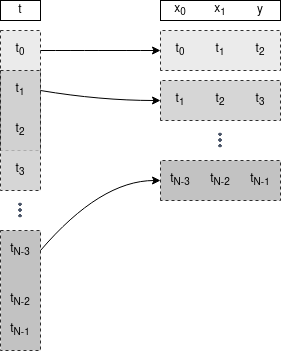
\includegraphics[width=3.0in]{img/sliding_window.png}
    \caption{Exemplo de aplicação do método de janelas deslizantes com passo $s=1$  para transformar a série temporal $t$ em uma matriz de características $X$ e um vetor alvo $y$. }
\end{figure}

Em alguns casos, também é possível utilizar outro parâmetro para a técnica, como o tamanho do passo da janela. No exemplo da Figura~\ref{fig:sliding_window_2}, esse tamanho de passo foi considerado como $s=1$, já que o tamanho do passo para formar cada registro foi de 1.

\begin{figure}[!ht] \label{fig:sliding_window_2}
    \centering
    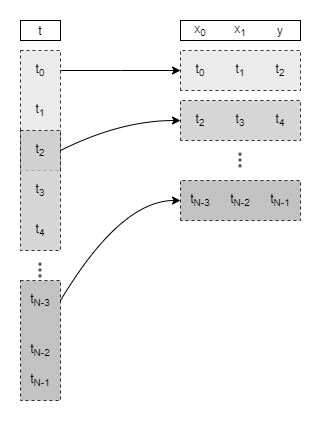
\includegraphics[width=3.0in]{img/sliding_window_2.png}
    \caption{Exemplo de aplicação do método de janelas deslizantes com passo $s=2$  para transformar a série temporal $t$ em uma matriz de características $X$ e um vetor alvo $y$. }
\end{figure}

É importante observar algumas características quanto ao método de janela deslizante, como a preservação da ordem dos registros, que é importante para garantir que a variável alvo será uma função dos dados anteriores na série temporal. Além disso, os primeiros $W$ valores da série temporal serão inutilizados, pois não possuem registros anteriores suficientes para gerar um registro na matriz de características.

A utilização deste método permite que o problema de previsão de séries temporais univariado seja resolvido como um problema de regressão supervisionado. Com os dados sendo transformados dessa forma, é possível aplicar qualquer algorítmo de regressão linear ou não linear de aprendizado de máquina.

Mesmo com a utilização desse método, os problemas relacionados à previsão de séries temporais como a flutuação de valores em um curto período. Para resolver esse tipo de problema, podem ser utilizados outros métodos, como o de médias móveis, que é explicado na Seção~\ref{sec:moving_average}.

\section{Média móvel} \label{sec:moving_average}
Existem alguns tipos de média móvel como a simples, a ponderada, a cumulativa, e a exponencial. Cada tipo de média móvel produz um efeito ao ser aplicada na série temporal, e podem ser usadas para alcançar objetivos diferentes. O algoritmo de média móvel simples, por exemplo, é utilizado para suavizar flutuações em curto prazo em uma série temporal, e consequentemente evidenciar tendências a longo prazo. Essa transformação se faz necessária, portanto, para facilitar o processo de aprendizado de modelos preditivos.

Para aplicar uma média móvel simples, dado uma sequência $P = (p_{1}, p_{2}, ..., p_{m})$ e um tamanho de janela $n$, é possível calcular cada valor $\overline{p}_{i}$ de média móvel conforme a Equação~\ref{eq:moving_average}.

\begin{equation} \label{eq:moving_average}
    \overline{p}_{i} = \dfrac{1}{n}\sum ^{i}_{j=i-n}p_{j}
\end{equation}

É possível notar que os primeiros $n$ valores da série temporal resultante são inviáveis de calcular, pois não possuem $n$ antecessores para o cáculo da média. Nesse sentido, uma abordagem simples é apenas desconsiderar os $n$ valores iniciais da série, já que em muitos casos o tamanho da série temporal é grande suficiente para essa perda não ser expressiva para os modelos preditivos.

\section{Regression WiSARD}
Conforme já apresentado no Capítulo~\ref{chap:03}, o modelo Regression WiSARD é utilizado para resolver problemas de regressão supervisionado. Dentre suas principais vantagens, estão a baixa utilização de memória e o baixo tempo de inferência. Utilizando os métodos apresentados na Seção~\ref{sec:sliding_window} e na Seção~\ref{sec:moving_average}, é possível, portanto, resolver um problema de previsão de série temporal com Regression WiSARD.

Para realizar tal tarefa, é necessário que os dados passem por um \textit{pipeline} de transformações, onde a ordem de tais transformações importa e é única. A Figura~\ref{fig:transforms_order} mostra um diagrama simples da ordem em que as trasnformações precisam ocorrer da esquerda para a direita. A técninca de médias móveis é a primeira a ser aplicada diretamente sobre a série temporal, e é responsável por suavizar flutuações a curto prazo, conforme explicado pela Seção~\ref{sec:moving_average}. Já a janela deslizante, apresentada na Seção~\ref{sec:sliding_window}, é aplicada sobre a série temporal de médias móveis, e é responsável pela transformação da série temporal em uma sequência de registros conforme um problema de regressão supervisionado. Por último, deve ser aplicada uma técnica de binarização sobre os dados, conforme explicado na Seção~\ref{sec:input_repr}, para que a representação da entrata seja compatível com a Regression WiSARD.

\begin{figure}[!ht] \label{fig:transforms_order}
    \centering
    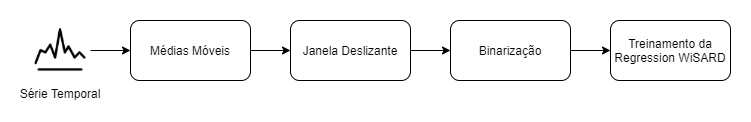
\includegraphics[width=5.0in]{img/transforms_order.png}
    \caption{}
\end{figure}

% Explicar predições com o modelo...
